% !TEX program = pdflatex
\documentclass[a4paper,14pt]{extarticle}

% ===== Язык и кодировка =====
\usepackage[T2A]{fontenc}
\usepackage[utf8]{inputenc}
\usepackage[russian,english]{babel}

% ===== Поля =====
\usepackage[left=30mm, right=15mm, top=20mm, bottom=20mm]{geometry}

% ===== Графика и таблицы =====
\usepackage{graphicx}
\usepackage{longtable}
\usepackage{array}
\usepackage{booktabs}
\usepackage{tabularx}
\usepackage{float}

% ===== Листинги кода =====
\usepackage{listings}
\usepackage{etoolbox}

\lstset{
  inputencoding=utf8,
  extendedchars=true,
  keepspaces=true,
  literate=
   {а}{{\selectfont\char224}}1 {б}{{\selectfont\char225}}1
   {в}{{\selectfont\char226}}1 {г}{{\selectfont\char227}}1
   {д}{{\selectfont\char228}}1 {е}{{\selectfont\char229}}1
   {ё}{{\"e}}1
   {ж}{{\selectfont\char230}}1 {з}{{\selectfont\char231}}1
   {и}{{\selectfont\char232}}1 {й}{{\selectfont\char233}}1
   {к}{{\selectfont\char234}}1 {л}{{\selectfont\char235}}1
   {м}{{\selectfont\char236}}1 {н}{{\selectfont\char237}}1
   {о}{{\selectfont\char238}}1 {п}{{\selectfont\char239}}1
   {р}{{\selectfont\char240}}1 {с}{{\selectfont\char241}}1
   {т}{{\selectfont\char242}}1 {у}{{\selectfont\char243}}1
   {ф}{{\selectfont\char244}}1 {х}{{\selectfont\char245}}1
   {ц}{{\selectfont\char246}}1 {ч}{{\selectfont\char247}}1
   {ш}{{\selectfont\char248}}1 {щ}{{\selectfont\char249}}1
   {ъ}{{\selectfont\char250}}1 {ы}{{\selectfont\char251}}1
   {ь}{{\selectfont\char252}}1 {э}{{\selectfont\char253}}1
   {ю}{{\selectfont\char254}}1 {я}{{\selectfont\char255}}1
   {А}{{\selectfont\char192}}1 {Б}{{\selectfont\char193}}1
   {В}{{\selectfont\char194}}1 {Г}{{\selectfont\char195}}1
   {Д}{{\selectfont\char196}}1 {Е}{{\selectfont\char197}}1
   {Ё}{{\"E}}1
   {Ж}{{\selectfont\char198}}1 {З}{{\selectfont\char199}}1
   {И}{{\selectfont\char200}}1 {Й}{{\selectfont\char201}}1
   {К}{{\selectfont\char202}}1 {Л}{{\selectfont\char203}}1
   {М}{{\selectfont\char204}}1 {Н}{{\selectfont\char205}}1
   {О}{{\selectfont\char206}}1 {П}{{\selectfont\char207}}1
   {Р}{{\selectfont\char208}}1 {С}{{\selectfont\char209}}1
   {Т}{{\selectfont\char210}}1 {У}{{\selectfont\char211}}1
   {Ф}{{\selectfont\char212}}1 {Х}{{\selectfont\char213}}1
   {Ц}{{\selectfont\char214}}1 {Ч}{{\selectfont\char215}}1
   {Ш}{{\selectfont\char216}}1 {Щ}{{\selectfont\char217}}1
   {Ъ}{{\selectfont\char218}}1 {Ы}{{\selectfont\char219}}1
   {Ь}{{\selectfont\char220}}1 {Э}{{\selectfont\char221}}1
   {Ю}{{\selectfont\char222}}1 {Я}{{\selectfont\char223}}1
}

\usepackage{xcolor}
\usepackage{fancyvrb}

% Предопределённый цвет: избегаем вычисления red!70!black на каждый символ
\colorlet{lststringcolor}{red!70!black}

\lstset{
  language=C,
  basicstyle=\footnotesize\ttfamily,
  keywordstyle=\color{blue}\bfseries,
  commentstyle=\color{gray}\itshape,
  stringstyle=\color{lststringcolor},
  numbers=left,
  numberstyle=\tiny\color{gray},
  numbersep=8pt,
  frame=single,
  breaklines=true,
  breakatwhitespace=false,
  columns=fullflexible,
  tabsize=4,
  showstringspaces=false,
  captionpos=b,
  postbreak=\mbox{$\hookrightarrow$\space},
}

% ===== Блок подсчёта операций =====
\newcommand{\opcount}[2]{%
  \par\vspace{2pt}%
  \noindent
  \colorbox{gray!15}{%
    \parbox{\dimexpr\linewidth-2\fboxsep\relax}{%
      \small\bfseries\ttfamily\raggedright #1:\enskip #2%
    }%
  }%
  \par\vspace{6pt}%
}

% ===== Гиперссылки =====
\PassOptionsToPackage{hyphens}{url}
\usepackage{amsmath}
\usepackage{hyperref}
\hypersetup{
  colorlinks=true,
  linkcolor=black,
  urlcolor=blue,
  citecolor=black,
}

% ===== Отступ первого абзаца =====
\usepackage{indentfirst}
\setlength{\parindent}{1.25cm}

% ===== Межстрочный интервал =====
\usepackage{setspace}
\onehalfspacing

% ===== Заголовки разделов =====
\usepackage{titlesec}
\titleformat{\section}{\normalfont\large\bfseries\centering}{\thesection.}{0.5em}{}
\titleformat{\subsection}{\normalfont\normalsize\bfseries}{\thesubsection.}{0.5em}{}

% ===== Перенос слов =====
\usepackage{ragged2e}
\emergencystretch=6em
\tolerance=9999
\hbadness=10001

% разрешить перенос длинных \texttt{...} на символах _ и /
\DeclareUrlCommand\code{\urlstyle{tt}}
\newcommand{\tcode}[1]{\code{#1}}

% ===== Подписи рисунков =====
\usepackage{caption}
\captionsetup{justification=centering, labelsep=endash}

\begin{document}

% ===================== ТИТУЛЬНЫЙ ЛИСТ =====================
\begin{titlepage}
\begin{center}

\textbf{Национальный исследовательский университет ИТМО}\\[0.5cm]
\textbf{Факультет безопасности информационных технологий}\\[2cm]

{\Large\textbf{Алгоритмы и структуры данных}}\\[1cm]
{\large Лабораторная работа №2}\\[0.5cm]
{\large\textbf{<<Цифровая сортировка с использованием кольцевой очереди>>}}\\[3cm]

\begin{flushright}
\begin{minipage}{0.45\textwidth}
\textbf{Выполнил:}\\
Студент группы N3247\\
Сивоконь А.А.\\[1cm]

\noindent\rule{6cm}{0.4pt}\\
\centerline{(подпись)}

\vspace{0.5cm}

\textbf{Преподаватель:}\\
Ерофеев С.А.\\[1cm]
\noindent\rule{6cm}{0.4pt}\\
\centerline{(отметка о выполнении)}

\vspace{1.5cm}

\noindent\rule{6cm}{0.4pt}\\
\centerline{(подпись)}
\end{minipage}
\end{flushright}

\vfill

Санкт-Петербург\\
2026

\end{center}
\end{titlepage}

% ===================== СОДЕРЖАНИЕ =====================
\newpage
\renewcommand{\contentsname}{Содержание}
\tableofcontents

% ===================== 1. ПОСТАНОВКА ЗАДАЧИ =====================
\newpage
\section{Постановка задачи}

\textbf{Цель работы:} разработать программу цифровой сортировки (Radix Sort LSD) для последовательности целых чисел (включая отрицательные), считываемых из файла, используя в качестве вспомогательной структуры данных \textbf{кольцевую очередь на основе односвязного списка}; определить сложность программы.

\vspace{0.5cm}
\textbf{Для достижения поставленной цели необходимо решить следующие задачи:}
\begin{enumerate}
  \item Реализовать кольцевую очередь на односвязном списке с операциями \texttt{enqueue}, \texttt{dequeue}, \texttt{queue\_is\_empty}, \texttt{queue\_free};
  \item Реализовать чтение массива целых чисел из файла;
  \item Реализовать алгоритм цифровой сортировки LSD через 10 кольцевых очередей-корзин;
  \item Корректно обработать отрицательные числа: разделить массив на части, отсортировать каждую независимо, объединить результат;
  \item Реализовать функцию вывода массива на экран;
  \item Оценить теоретическую сложность алгоритма;
  \item Провести тестирование программы на различных наборах данных;
  \item Составить блок-схемы алгоритма и оформить отчёт.
\end{enumerate}

% ===================== 2. ОПИСАНИЕ АЛГОРИТМА =====================
\newpage
\section{Описание алгоритма сортировки}

\subsection{Кольцевая очередь на односвязном списке}

В качестве вспомогательной структуры данных используется кольцевая очередь на основе динамически выделяемых узлов:

\begin{itemize}
  \item Узел \texttt{Node} содержит значение \texttt{value} и указатель \texttt{next} на следующий узел.
  \item Очередь \texttt{Queue} хранит указатель \texttt{tail} на \textit{хвостовой} узел и счётчик \texttt{size}. Голова очереди доступна как \texttt{tail->next}. Такая организация обеспечивает $O(1)$ как для вставки (\texttt{enqueue}), так и для извлечения (\texttt{dequeue}).
  \item При добавлении первого элемента узел замыкается на себя: \texttt{node->next = node}.
\end{itemize}

\textbf{Операции и их сложность:}

\begin{center}
\begin{tabular}{|l|l|l|}
\hline
\textbf{Функция} & \textbf{Описание} & \textbf{Операций} \\
\hline
\texttt{queue\_init}      & инициализировать поля \texttt{tail=NULL}, \texttt{size=0} & 8 \\
\hline
\texttt{queue\_is\_empty} & вернуть \texttt{size==0}                                  & 4 \\
\hline
\texttt{enqueue}          & добавить элемент в хвост                                  & 23 / 30 \\
\hline
\texttt{dequeue}          & извлечь элемент из головы                                 & 26 \\
\hline
\texttt{queue\_free}      & освободить все узлы                                       & $15 + 6n$ \\
\hline
\end{tabular}
\end{center}

Для \texttt{enqueue}: 23 операции~--- первый элемент (узел замыкается на себя), 30~--- все последующие (вставка в непустую очередь).

\subsection{Алгоритм цифровой сортировки LSD}

Цифровая сортировка~--- нерекурсивный алгоритм, обрабатывающий числа поразрядно. В варианте LSD (Least Significant Digit) обработка ведётся от \textit{младшего} разряда к \textit{старшему}.

\textbf{Пошаговый алгоритм функции \tcode{counting_sort_by_queue}:}

\begin{enumerate}
  \item \textbf{Шаг 1.} Инициализировать 10 кольцевых очередей \texttt{buckets[0..9]}.
  \item \textbf{Шаг 2.} Для каждого элемента вычислить цифру текущего разряда: \texttt{(arr[i] / exp) \% 10}; выполнить \texttt{enqueue} в соответствующую корзину~\texttt{buckets[digit]}.
  \item \textbf{Шаг 3.} Обходя корзины \texttt{buckets[0..9]} по порядку, последовательно извлекать элементы через \texttt{dequeue} и записывать обратно в \texttt{arr[]}. Порядок FIFO внутри каждой корзины гарантирует устойчивость сортировки.
  \item \textbf{Шаг 4.} Освободить все 10 очередей (\texttt{queue\_free}).
\end{enumerate}

\textbf{Подсчёт операций одного прохода} ($k = 10$, 7 типов операций: вызов, возврат, переход по ссылке, присваивание, сравнение, арифметика, индексация):

\begin{center}
\begin{tabular}{|l|l|r|}
\hline
\textbf{Шаг} & \textbf{Формула} & \textbf{k=10} \\
\hline
1. Инициализация очередей                          & $11k + 2$            & 112 \\
\hline
2. Распределение по корзинам (enqueue)             & $12n + 2$            & $12n+2$ \\
\hline
3. Сбор из корзин (dequeue) $+$ \texttt{idx=0}     & $1 + (3k+2) + 4(n+k) + 7n$ & $11n+45$ \\
\hline
4. Освобождение очередей (queue\_free)             & $6n + 11k + 2$       & $6n+112$ \\
\hline
\textbf{Итого}                                     & $\mathbf{29n + 29k + 9}$ & $\mathbf{29n + 299}$ \\
\hline
\end{tabular}
\end{center}

\textit{Примечание.} В анализе \texttt{radix\_sort\_nonneg} стоимость одного прохода принята как $23n + 187$~--- без учёта фазы освобождения очередей (шаг~4), которая учитывается отдельно:

\[
  T_{1\,\text{прохода}} = 23n + 187 \quad (k{=}10)
\]
\[
  T_{\text{radix\_sort\_nonneg}} = \underbrace{(7n+14)}_{\text{find\_max} + \text{служ.}}
    + \underbrace{(4d+5)}_{\text{цикл по exp}}
    + d\cdot(23n + 187)
    = 23d\cdot n + 191d + 7n + 19
\]

\textbf{Поддержка отрицательных чисел.} Функция \texttt{radix\_sort} разделяет массив на два подмассива~--- отрицательных (по абсолютному значению) и неотрицательных,~--- сортирует каждый через \texttt{radix\_sort\_nonneg}, затем объединяет: сначала отрицательные в обратном порядке, затем положительные.

\textbf{Оценка сложности алгоритма:}
\begin{itemize}
  \item Временная: $O(d \cdot n)$, где $n$~--- количество элементов, $d$~--- число разрядов в максимальном числе по модулю. При фиксированном $d$ сложность \textbf{линейная}: $O(n)$.
  \item Пространственная: $O(n)$~--- на одном проходе суммарно выделяется $n$ узлов \texttt{Node}; после сбора они освобождаются.
\end{itemize}

\subsection{Маршрут программы}

\begin{enumerate}
  \item \textbf{Чтение входного файла} (\texttt{read\_file}): двухпроходное чтение~--- сначала подсчёт числа элементов, затем выделение массива и считывание значений.
  \item \textbf{Вывод исходного массива} (\texttt{print\_array}).
  \item \textbf{Выполнение Radix Sort} (\texttt{radix\_sort}): разделение на отрицательные/неотрицательные, сортировка, объединение.
  \item \textbf{Вывод отсортированного массива} (\texttt{print\_array}).
  \item \textbf{Вывод оценки сложности:} $n$, максимальный элемент по модулю, $d$, $k$, число операций по формуле $T = 23d\cdot n + 191d + 7n + 19$, число дополнительных ячеек памяти (узлов очереди).
  \item \textbf{Освобождение памяти}: \texttt{free(arr)}.
\end{enumerate}

% ===================== 3. ОПИСАНИЕ ПЕРЕМЕННЫХ =====================
\newpage
\section{Описание используемых переменных}

В таблице~\ref{tab:vars} приведено описание переменных программы.

\captionsetup[longtable]{name={Таблица}}

\newcolumntype{L}[1]{>{\RaggedRight\arraybackslash}p{#1}}

\begin{longtable}{|L{3.4cm}|L{3.0cm}|L{3.6cm}|L{4.5cm}|}
\caption{Описание переменных программы}\label{tab:vars}\\
\hline
\textbf{Переменная} & \textbf{Тип} & \textbf{Границы} & \textbf{Назначение} \\
\hline
\endfirsthead
\hline
\textbf{Переменная} & \textbf{Тип} & \textbf{Границы} & \textbf{Назначение} \\
\hline
\endhead
\hline
\endfoot

\multicolumn{4}{|c|}{\textbf{Главная программа (main.c)}} \\
\hline
filename & \texttt{const char*}  & строка               & Имя входного файла \\
\hline
arr      & \texttt{int*}         & адрес                & Указатель на массив \\
\hline
n        & \texttt{int}          & $[1;\;2^{31}-1]$     & Количество прочитанных чисел \\
\hline
max\_val & \texttt{int}          & $[0;\;2^{31}-1]$     & Максимальное значение по модулю \\
\hline
d        & \texttt{int}          & $[1;\;10]$           & Число разрядов \texttt{max\_val} \\
\hline
tmp      & \texttt{int}          & $[1;\;2^{31}-1]$     & Временная для подсчёта разрядов \\
\hline
ops      & \texttt{int}          & $\geq 0$             & Расчётное число операций \\
\hline
v        & \texttt{int}          & $[0;\;2^{31}-1]$     & $|\texttt{arr[i]}|$ при поиске \texttt{max\_val} \\
\hline

\multicolumn{4}{|c|}{\textbf{Кольцевая очередь (radix\_sort.c)}} \\
\hline
Node.value  & \texttt{int}        & любое целое          & Хранимое значение узла \\
\hline
Node.next   & \texttt{Node*}      & адрес                & Указатель на следующий узел \\
\hline
Queue.tail  & \texttt{Node*}      & адрес / NULL         & Хвостовой узел очереди \\
\hline
Queue.size  & \texttt{int}        & $[0;\;n]$            & Текущий размер очереди \\
\hline
head        & \texttt{Node*}      & адрес                & Головной узел (\texttt{tail->next}) \\
\hline
cur         & \texttt{Node*}      & адрес                & Текущий узел в \texttt{queue\_free} \\
\hline

\multicolumn{4}{|c|}{\textbf{Ввод/вывод (radix\_sort.c)}} \\
\hline
fp    & \texttt{FILE*}  & адрес             & Указатель на открытый файл \\
\hline
n     & \texttt{int}    & $[1;\;2^{31}-1]$  & Счётчик при первом проходе \\
\hline
tmp   & \texttt{int}    & любое целое       & Значение при счёте чисел \\
\hline
i     & \texttt{int}    & $[0;\;n-1]$       & Индекс цикла второго прохода \\
\hline

\multicolumn{4}{|c|}{\textbf{Цифровая сортировка (radix\_sort.c)}} \\
\hline
exp           & \texttt{int}       & $\{1, 10, \ldots, 10^{d-1}\}$  & Текущий разряд \\
\hline
buckets[10]   & \texttt{Queue[10]} & ---                   & Массив из 10 корзин-очередей \\
\hline
digit         & \texttt{int}       & $[0;\;9]$             & Цифра текущего разряда \\
\hline
idx           & \texttt{int}       & $[0;\;n-1]$           & Индекс вставки при сборе \\
\hline
max           & \texttt{int}       & $[0;\;2^{31}-1]$      & Текущий максимум в \texttt{find\_max} \\
\hline
neg\_n        & \texttt{int}       & $[0;\;n]$             & Количество отрицательных чисел \\
\hline
pos\_n        & \texttt{int}       & $[0;\;n]$             & Количество неотрицательных чисел \\
\hline
neg           & \texttt{int*}      & адрес                 & Абс.\ значения отрицательных \\
\hline
pos           & \texttt{int*}      & адрес                 & Неотрицательные числа \\
\hline
ni, pi        & \texttt{int}       & $[0;\;n-1]$           & Индексы заполнения \texttt{neg}/\texttt{pos} \\
\hline

\end{longtable}

% ===================== 4. ТЕСТИРОВАНИЕ =====================
\newpage
\section{Тестирование программы}

Для тестирования использовался файл \texttt{input.txt}:
\begin{Verbatim}[frame=single,fontsize=\footnotesize]
170 45 75 90 802 24 2 66
\end{Verbatim}

\subsection{Тест 1: стандартная сортировка (положительные числа)}

\begin{Verbatim}[frame=single,fontsize=\footnotesize]
$ ./sort input.txt

Чтение файла 'input.txt'...
Прочитано 8 чисел.

Исходный массив:
170 45 75 90 802 24 2 66

Выполняем Radix Sort...
Отсортированный массив:
2 24 45 66 75 90 170 802

── Оценка сложности ─────────────────────────────
  n (элементов)           8
  max элемент             802
  d (разрядов)            3
  k (основание, BASE)     10
  Операций:              1200
  Доп. ячеек (узлов):    8
─────────────────────────────────────────────────
\end{Verbatim}

Массив успешно отсортирован. Операций: $23\cdot3\cdot8 + 191\cdot3 + 7\cdot8 + 19 = 1200$.

\subsection{Тест 2: массив с отрицательными числами}

Входной файл \texttt{neg.txt}: \texttt{-15 3 -7 42 -2 18}

\begin{Verbatim}[frame=single,fontsize=\footnotesize]
$ ./sort neg.txt

Чтение файла 'neg.txt'...
Прочитано 6 чисел.

Исходный массив:
-15 3 -7 42 -2 18

Выполняем Radix Sort...
Отсортированный массив:
-15 -7 -2 3 18 42

── Оценка сложности ─────────────────────────────
  n (элементов)           6
  max элемент             42
  d (разрядов)            2
  k (основание, BASE)     10
  Операций:              719
  Доп. ячеек (узлов):    6
─────────────────────────────────────────────────
\end{Verbatim}

Программа корректно разделила массив на подмассивы отрицательных ($[-15,\,-7,\,-2]$ по модулю) и неотрицательных ($[3,\,18,\,42]$) чисел, отсортировала каждый и объединила результат.

\subsection{Тест 3: несуществующий файл}

\begin{Verbatim}[frame=single,fontsize=\footnotesize]
$ ./sort missing.txt

Чтение файла 'missing.txt'...
Ошибка: не удалось открыть файл 'missing.txt'
\end{Verbatim}

Программа корректно обрабатывает ошибку открытия файла и завершает работу с кодом \texttt{EXIT\_FAILURE}.

\subsection{Тест 4: пустой файл}

Файл \texttt{empty.txt} предварительно очищен:

\begin{Verbatim}[frame=single,fontsize=\footnotesize]
$ ./sort empty.txt

Чтение файла 'empty.txt'...
Ошибка: файл 'empty.txt' пуст или не содержит чисел
\end{Verbatim}

Программа корректно обнаруживает пустой файл и завершает работу с кодом \texttt{EXIT\_FAILURE}.

% ===================== 5. БЛОК-СХЕМЫ =====================
\newpage
\section{Блок-схемы алгоритма}

Блок-схемы всех подпрограмм приведены в Приложении~А (стр.~\pageref{sec:appendix}).

Перечень блок-схем:
\begin{enumerate}
  \item Главная программа (\texttt{main})
  \item Чтение из файла (\texttt{read\_file})
  \item Цифровая сортировка (\texttt{radix\_sort})
  \item Сортировка по разряду через очереди (\tcode{counting_sort_by_queue})
  \item Добавление элемента в очередь (\texttt{enqueue})
  \item Извлечение элемента из очереди (\texttt{dequeue})
\end{enumerate}

% ===================== 6. ИСХОДНЫЙ КОД =====================
\newpage
\section{Исходный код программы}

Программа состоит из трёх файлов: \texttt{main.c}~--- точка входа, ввод/вывод и вычисление сложности; \texttt{radix\_sort.h}~--- объявления функций; \texttt{radix\_sort.c}~--- реализация кольцевой очереди и алгоритма сортировки.

% -------- 6.1 main.c --------
\subsection{Файл main.c}

\lstinputlisting[language=C]{main.c}
\opcount{read\_file}{$16n + 21$ операций; \textbf{сложность:} $O(n)$}
\opcount{print\_array}{$8n + 3$ операций; \textbf{сложность:} $O(n)$}
\opcount{main}{прямые операции: $12n + 5d + 35$; итого c вызовами: $T \approx 23d\cdot n + 387d + 69n + 136$; \textbf{сложность:} $O(d \cdot n)$}

% -------- 6.2 radix\_sort.h --------
\subsection{Файл radix\_sort.h}

\lstinputlisting[language=C]{radix_sort.h}

% -------- 6.3 radix\_sort.c --------
\subsection{Файл radix\_sort.c}

\subsubsection*{Кольцевая очередь}

\lstinputlisting[language=C, firstline=1, lastline=91]{radix_sort.c}
\opcount{queue\_init}{8 операций (3+3+1+1); \textbf{сложность:} $O(1)$}
\opcount{queue\_is\_empty}{4 операции (2 ссылки + 1 сравн. + 1 возврат); \textbf{сложность:} $O(1)$}
\opcount{enqueue}{23 операции (первый эл.) / 30 операций (последующие); \textbf{сложность:} $O(1)$}
\opcount{dequeue}{26 операций (нормальный путь); \textbf{сложность:} $O(1)$}
\opcount{queue\_free}{$15 + 6n$ операций; \textbf{сложность:} $O(n)$}

\subsubsection*{Вспомогательные функции и сортировка}

\lstinputlisting[language=C, firstline=93, lastline=213]{radix_sort.c}
\opcount{find\_max}{$7n + 5$ операций; \textbf{сложность:} $O(n)$}
\opcount{counting\_sort\_by\_queue}{$23n + 187$ операций ($k{=}10$, без учёта queue\_free); \textbf{сложность:} $O(n)$}
\opcount{radix\_sort\_nonneg}{$23d\cdot n + 191d + 7n + 19$ операций; \textbf{сложность:} $O(d \cdot n)$}
\opcount{radix\_sort}{общий случай: $23d\cdot n + 382d + 25n + 9\cdot n_- + 8\cdot n_+ + 74$ (где $n_-$/$n_+$~--- кол-во отр./пол.\ чисел); \textbf{сложность:} $O(d \cdot n)$}

% ===================== ЗАКЛЮЧЕНИЕ =====================
\newpage
\section*{Заключение}
\addcontentsline{toc}{section}{Заключение}

В ходе выполнения лабораторной работы была разработана программа на языке~C, реализующая цифровую сортировку LSD целых чисел (включая отрицательные), считываемых из файла, с использованием кольцевых очередей на основе односвязного списка в качестве вспомогательных структур данных.

Программа организована в три файла: \texttt{main.c} содержит точку входа, ввод/вывод и расчёт сложности; \texttt{radix\_sort.h} объявляет функции; \texttt{radix\_sort.c} реализует кольцевую очередь и алгоритм сортировки.

Поддержка отрицательных чисел реализована через разделение массива на подмассивы отрицательных (преобразованных в модули) и неотрицательных, их независимую сортировку и последующее объединение.

Теоретическая сложность алгоритма составляет $O(d \cdot n)$ по времени и $O(n)$ по памяти. При фиксированном $d$ алгоритм работает за \textbf{линейное} время $O(n)$. По сравнению с реализацией через вспомогательный массив (ЛР~1, $26n + 120$ операций на проход), линейный коэффициент ниже ($23n$ против $26n$), однако константа выше ($187$ против $120$) из-за накладных расходов инициализации и освобождения 10~очередей на каждый проход. Асимптотика остаётся той же: $O(d \cdot n)$.

Результаты тестирования подтверждают корректность сортировки для положительных и отрицательных чисел, а также правильную обработку ошибочных ситуаций.

% ===================== ПРИЛОЖЕНИЕ А =====================
\newpage
\phantomsection
\label{sec:appendix}
\section*{Приложение А. Блок-схемы алгоритма}
\addcontentsline{toc}{section}{Приложение А. Блок-схемы алгоритма}

\begin{figure}[p]
\renewcommand{\figurename}{Рис.}
\centering

\includegraphics[width=\textwidth,height=0.92\textheight,keepaspectratio]{flowcharts/1_main.png}
\caption{Главная программа (main)}
\end{figure}

\begin{figure}[p]
\renewcommand{\figurename}{Рис.}
\centering

\includegraphics[width=\textwidth,height=0.92\textheight,keepaspectratio]{flowcharts/2_read_file.png}
\caption{Чтение из файла (read\_file)}
\end{figure}

\begin{figure}[p]
\renewcommand{\figurename}{Рис.}
\centering

\includegraphics[width=\textwidth,height=0.92\textheight,keepaspectratio]{flowcharts/3_radix_sort.png}
\caption{Цифровая сортировка (radix\_sort)}
\end{figure}

\begin{figure}[p]
\renewcommand{\figurename}{Рис.}
\centering
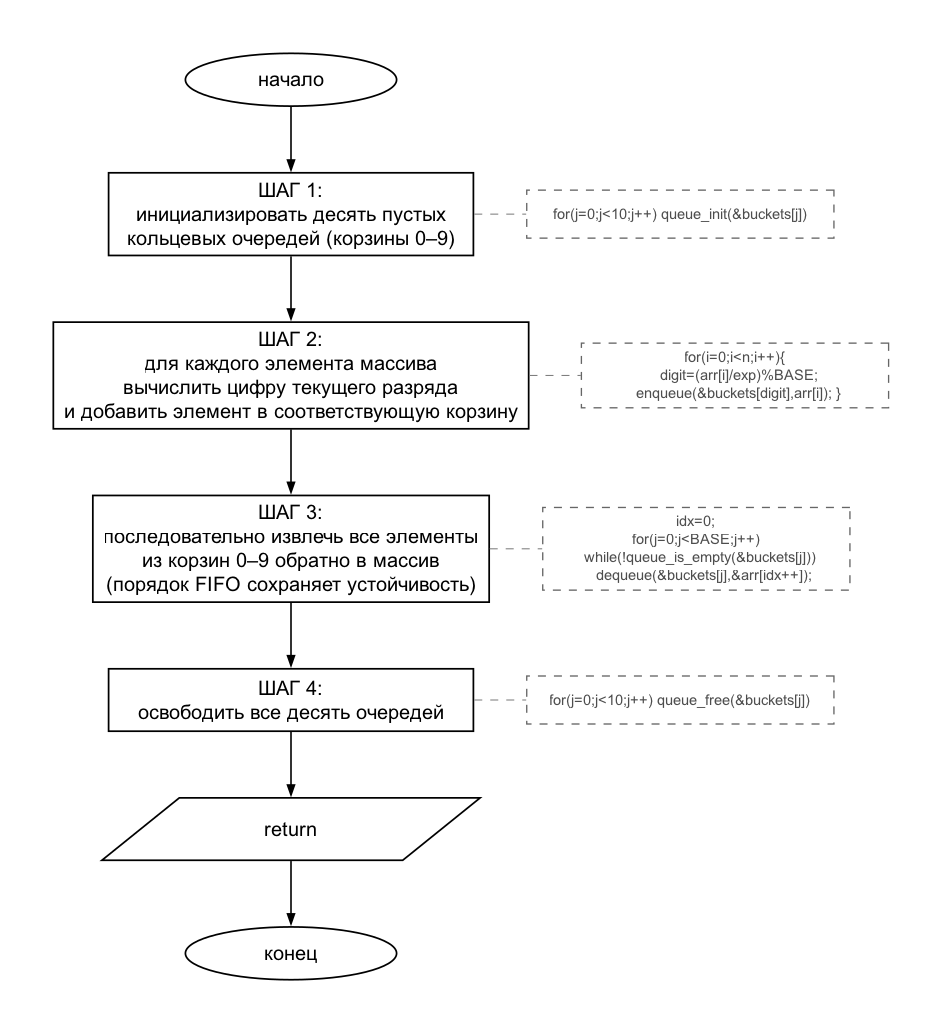
\includegraphics[width=\textwidth,height=0.92\textheight,keepaspectratio]{flowcharts/4_counting_sort_queue.png}
\caption{Сортировка по разряду через очереди (counting\_sort\_by\_queue)}
\end{figure}

\begin{figure}[p]
\renewcommand{\figurename}{Рис.}
\centering
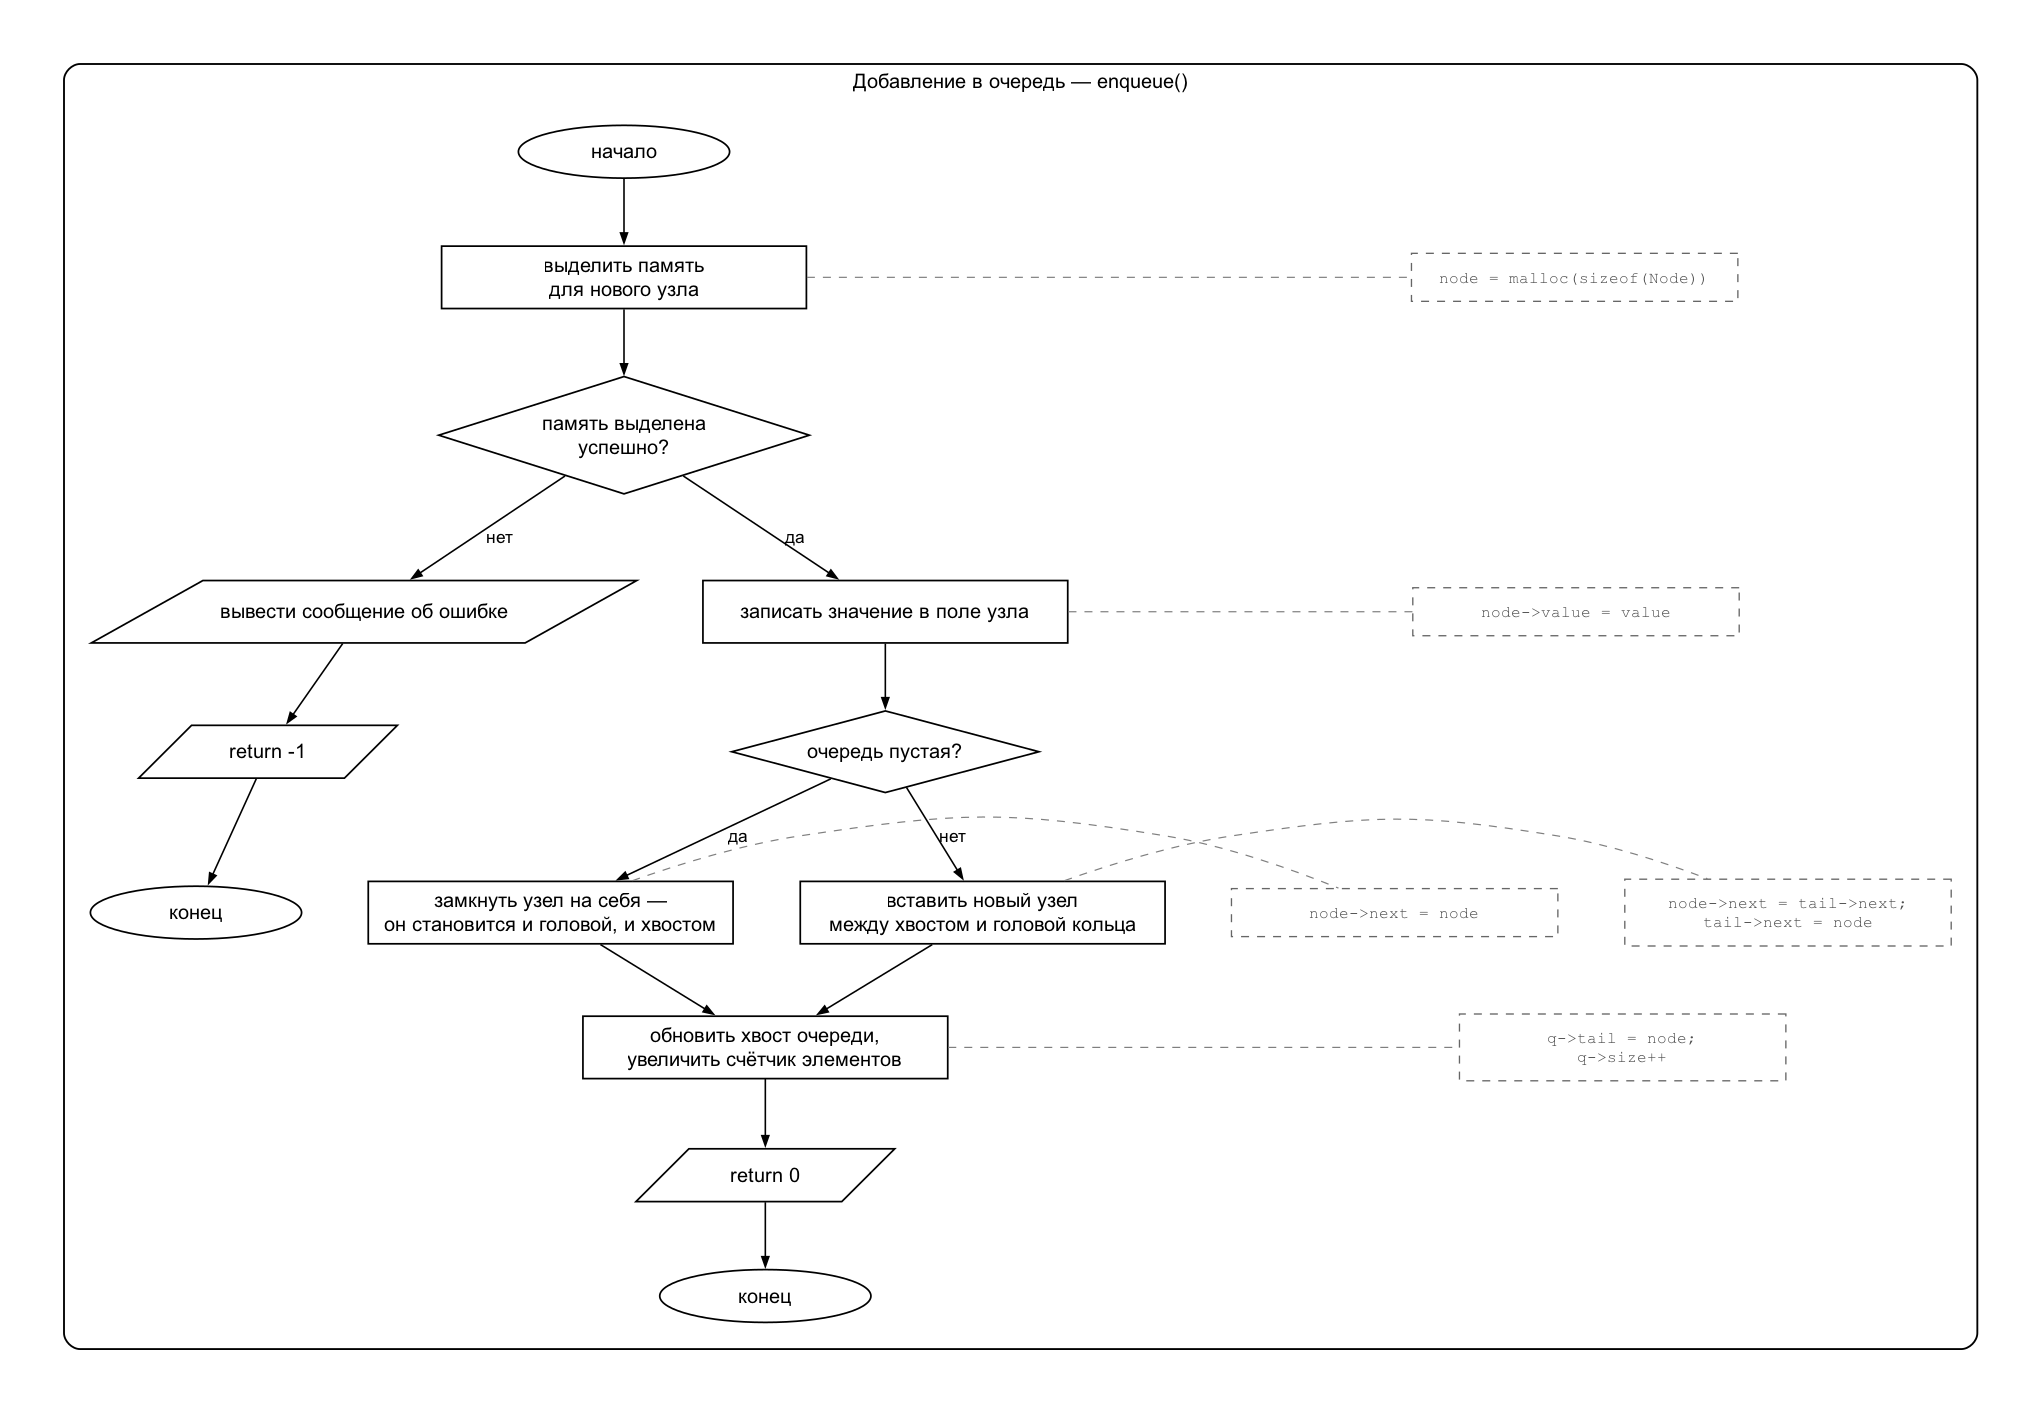
\includegraphics[width=\textwidth,height=0.92\textheight,keepaspectratio]{flowcharts/5a_enqueue.png}
\caption{Добавление элемента в очередь (enqueue)}
\end{figure}

\begin{figure}[p]
\renewcommand{\figurename}{Рис.}
\centering
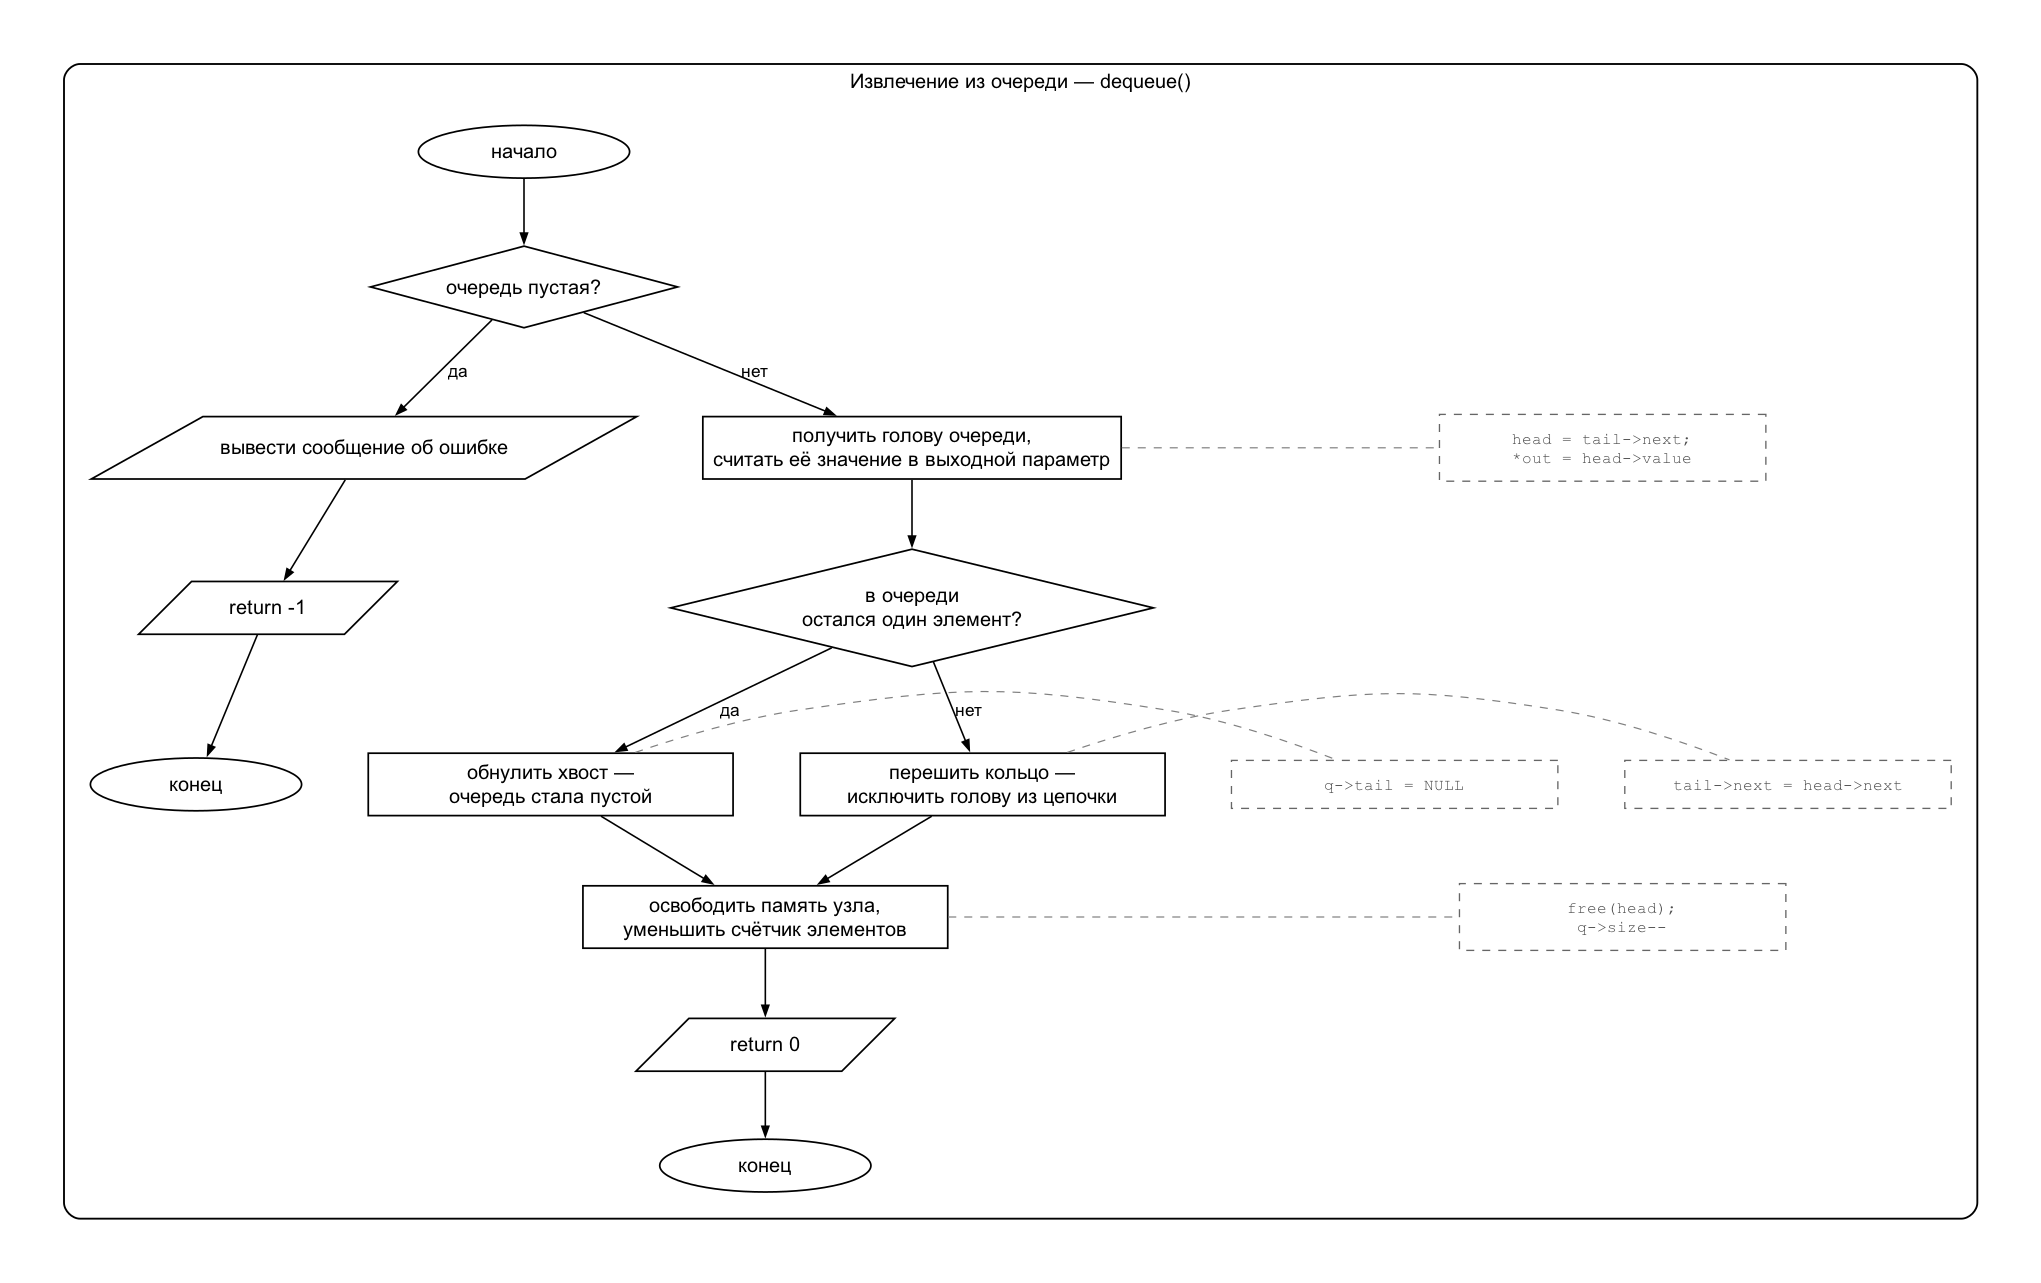
\includegraphics[width=\textwidth,height=0.92\textheight,keepaspectratio]{flowcharts/5b_dequeue.png}
\caption{Извлечение элемента из очереди (dequeue)}
\end{figure}

\end{document}
